\documentclass[11pt,a4paper,oneside,titlepage]{article}
%the document class has to be on the top line. The options, in the square brackets are fairly self-explanitory...
%lines starting with a percentage symbol are comments and won't be read buy the LaTeX package.
\usepackage[authoryear,sectionbib,round]{natbib} 
\usepackage[dvips]{graphicx} 
\usepackage{sidecap}
\bibliographystyle{abbrvnat} 
\usepackage{fancyhdr}
\usepackage{placeins}
\usepackage{subfigure}
\usepackage{timet}
\setlength{\topmargin}{-1.0cm}
\setlength{\textheight}{24.5cm}
\setlength{\oddsidemargin}{+0.2cm}
\setlength{\textwidth}{15.6cm}
\renewcommand{\textfraction}{0.1}
\renewcommand{\topfraction}{0.9}
\renewcommand{\bottomfraction}{0.9}
\renewcommand{\floatpagefraction}{0.80}
\textfloatsep 15pt
\setlength{\intextsep}{.5cm}
\addtolength{\abovecaptionskip}{-.1cm}
\renewcommand{\headrulewidth}{0.4pt}
\renewcommand{\footrulewidth}{0.4pt}

%two backslashes will start a new line
\title{\Huge First Year Report: \\
Seismological observations \\
of the inner core }
\author{ Jessica Irving \\
         Trinity College}
\date{}
\pagestyle{fancy}
\lhead{}
\chead{}
\rhead{First Year Report}
\lfoot{Your Name}
\cfoot{}
\rfoot{\thepage}

%Actual document begins here.
\begin{document}

\maketitle
% this will automatically make the title with the info above. It will default to today's date, to have no date put \date{} above here.

\tableofcontents
% This command automatically list all the sections, subsections, and subsubsections, together with their pagenumbers

\newpage
%to force LaTeX to use a new page use this. (use sparingly as LaTeX knows best!)



\section{Abstract}

An abstract summary of my material. I would like to use this section to lure any potential readers into looking at this exciting treatise on my research topic. I've also been told that in the abstract it's best not to use \emph{bold}, \textit{italics} ,  type \underline{underlined text} or anything else that's too fancy. So maybe I shouldn't have. I've left text I wrote in the rest of this - but that doesn't mean it's worth reading.


\begin{figure}[bth]
\begin{center}
% Lots of different options could be inclulded here eg rotate. 
% ps or epsi images are the easiest to include. The .eps format 
% gives a preview of the image which is sometimes missing for 
%.ps images in some dvi viewers. to convert between the two use ps2eps.
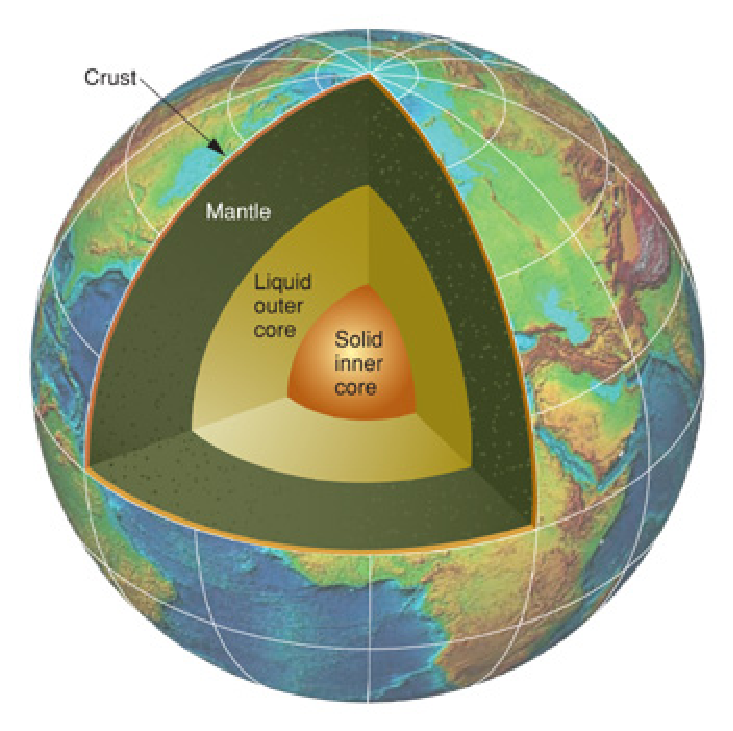
\includegraphics[width=8cm]{fried.eps}
\caption{\small The basic structure of the Earth.}
\label{fig:Earth}
\end{center}
\end{figure}

\section{Introduction}

The Earth has lots of layers - have a look at Figure~\ref{fig:Earth} to see what they might be. And be aware that this figure is not to scale - though it is pretty. %When you have used the \label{fig:Earth} command in the figure above, every time you would like to refer




\subsection{Making lists}
%an example subsection

Should you need to make lists you can:
\begin{enumerate}
\item list your 
\item points by numbering them
\item without having to change all the numbers if
\item you add a new point in the middle or
\item you rearrange them.
\end{enumerate}

\begin{itemize}
\item On the other hand you may
\item prefer to just have your 
\item objects without numbers
\item and just put bullet points by them
\end{itemize}

\subsection{Typing as vertabim}

The \verb|\verb| command will print the text exactly as you type it, without the pretty \LaTeX formatting.~\footnote{a short comment added hear will appear in a footnote to this page}. ``trees''.

\subsubsection{Some more text}
However, for waves of very low frequencies and long wavelengths, effects like gravitation, ellipticity and rotation of the Earth become important and the approximations used in the ray theory are invalidated. The best way to model these seismic waves is using normal modes. Normal modes are free oscillations of the whole Earth. The vertical and horizontal motion they cause at the Earth's surface can be detected using a seismograph. for asummary of recent research see Song's review~\cite{song97}.  % refer to a paper included in the bibliography file using it's key - in this case ``song97''. This will then cite the authors and year for you - change the natbib options in the preamble to get a different citation style.


\section{Theory}

\subsection{Coupling of normal modes}
The Earth is not a perfect sphere, but an oblate spheroid - the radius of the Earth at the poles is 6357km and 6378km at the equator. The asphericity and rotation of the Earth remove the degeneracy of the normal modes. The mode is now a set of $(2l+1)$ singlets. 

% a little maths is included here and some more below. 
\begin{equation} \label{eq:misfit}
\mathrm{misfit} = \frac {\left|z_d - z_s\right| ^2}{z_d^2}
\end{equation}
where $z_d$ is the complex value of the data trace and $z_s$ is the complex
value of the synthetic seismogram trace.




\begin{table}
\begin{center}
\caption{Groups of inner core modes that couple with the seven modes of interest in the Woodhouse model.}
\begin{tabular}{|l|l|}
\hline
Mode Studied & Couples With \\
\hline
$_2S_0$ & $_7S_2$ $_6S_2$ $_4S_6$ \\
$_{11}S_1$ & $_{10}S_1$ $_9S_3$ $_7S_5$ \\
$_4S_0$ & $_{10}S_2$ $_{11}S_2$ \\
\hline
\end{tabular}
\end{center}
\end{table}





\section{Conclusions}

It has been shown that when inner core anisotropy is taken into account the difference between the self and full coupling approximation can be large. This is due to the coupling of inner core modes with degree zero, two or four difference in order.


%together with the file shortbib.bib this command will let BiBTeX makea nice bibliography. the style can be varied by changing the command ``\bibliographystyle'' at the top of the document.

\bibliography{shortbib}

%This changes the section numbering to appendix lettering

\appendix

\section{Appendix - Theory for normal modes}

The displacement of the Earth, $\mathbf{s}$, can be represented by:

\begin{equation}\label{eq:S}
\mathbf{Hs} + \mathbf{W}\partial_t \mathbf{s} + \mathbf{P}\partial_t^2
\mathbf{s} = \mathbf{S}
\end{equation}

Where $\mathbf{H}$ represents the potential energy operator, $\mathbf{W}$ represents the Coriolis operator, $\mathbf{P}$ is the kinetic energy operator and $\mathbf{S}$ represents the excitation caused by the earthquake source. The solution to this equation will be of the form $s(x,t) = s(x)e^{\imath \omega t}$ where $\omega$ is the radial frequency of the normal mode.


\end{document}


%anything written after here won't make it into the document;
even if it's not commented out!


